\subsection{User Interfaces}
\label{subsec:user_interfaces}

Below are the main screenshots of the application. 
The first ones show the features available to both logged-in users and anonymous visitors, such as the homepage and the public path search.

\begin{figure}[H]
        \centering
        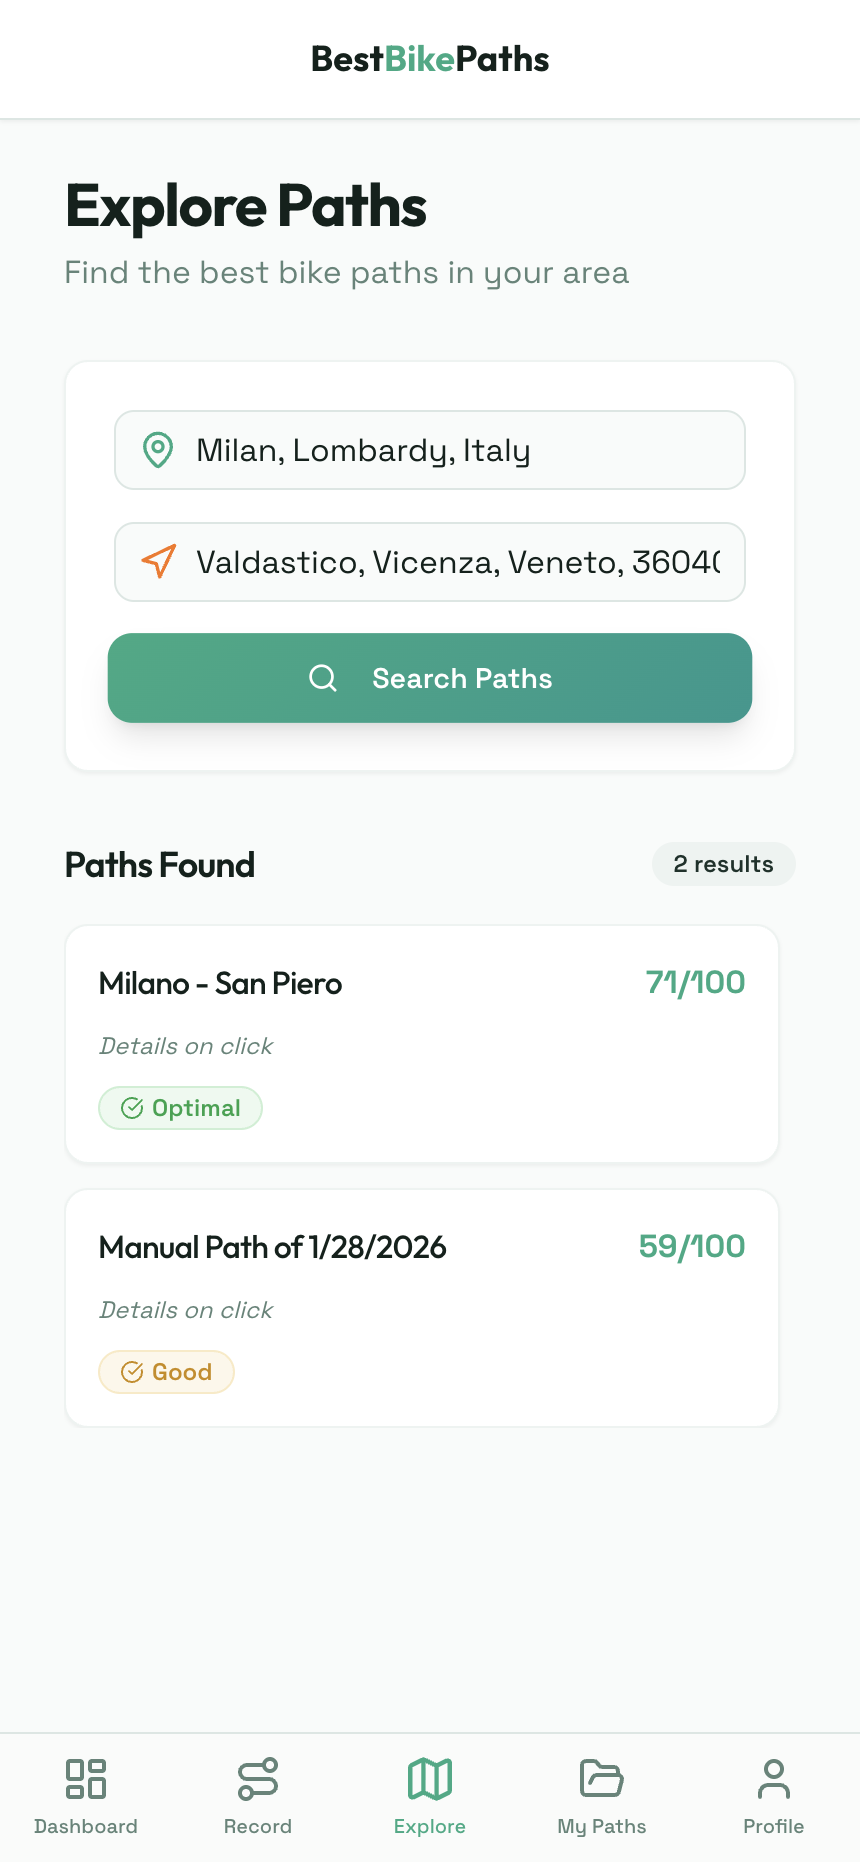
\includegraphics[width=0.25\textwidth]{Images/explore_paths_def.png}
        \caption{Public path search}
    \label{fig:public_path_search}
\end{figure}

The following screens are accessible only after authentication: the profile page, the activity recording interface, and the section where users can view their personal paths, both public and private.

\begin{figure}[H]
        \centering
        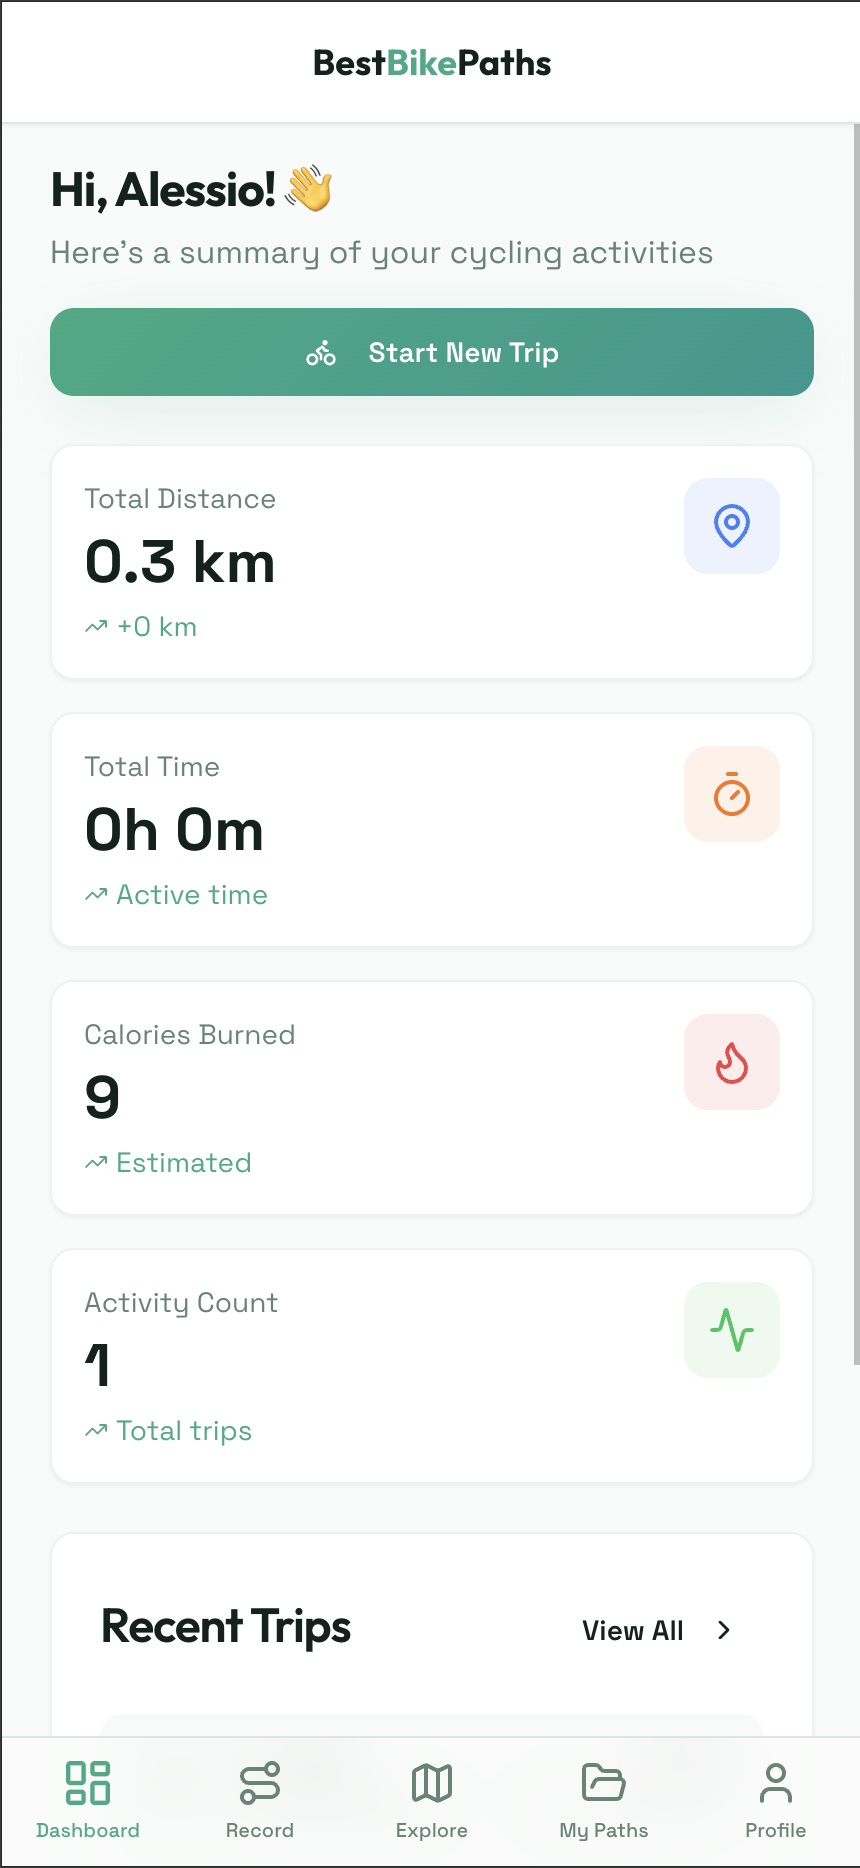
\includegraphics[width=0.25\textwidth]{Images/dashboard_def.png}
        \caption{Dashboard}
    \label{fig:dashboard}
\end{figure}

\begin{figure}[H]
        \centering
        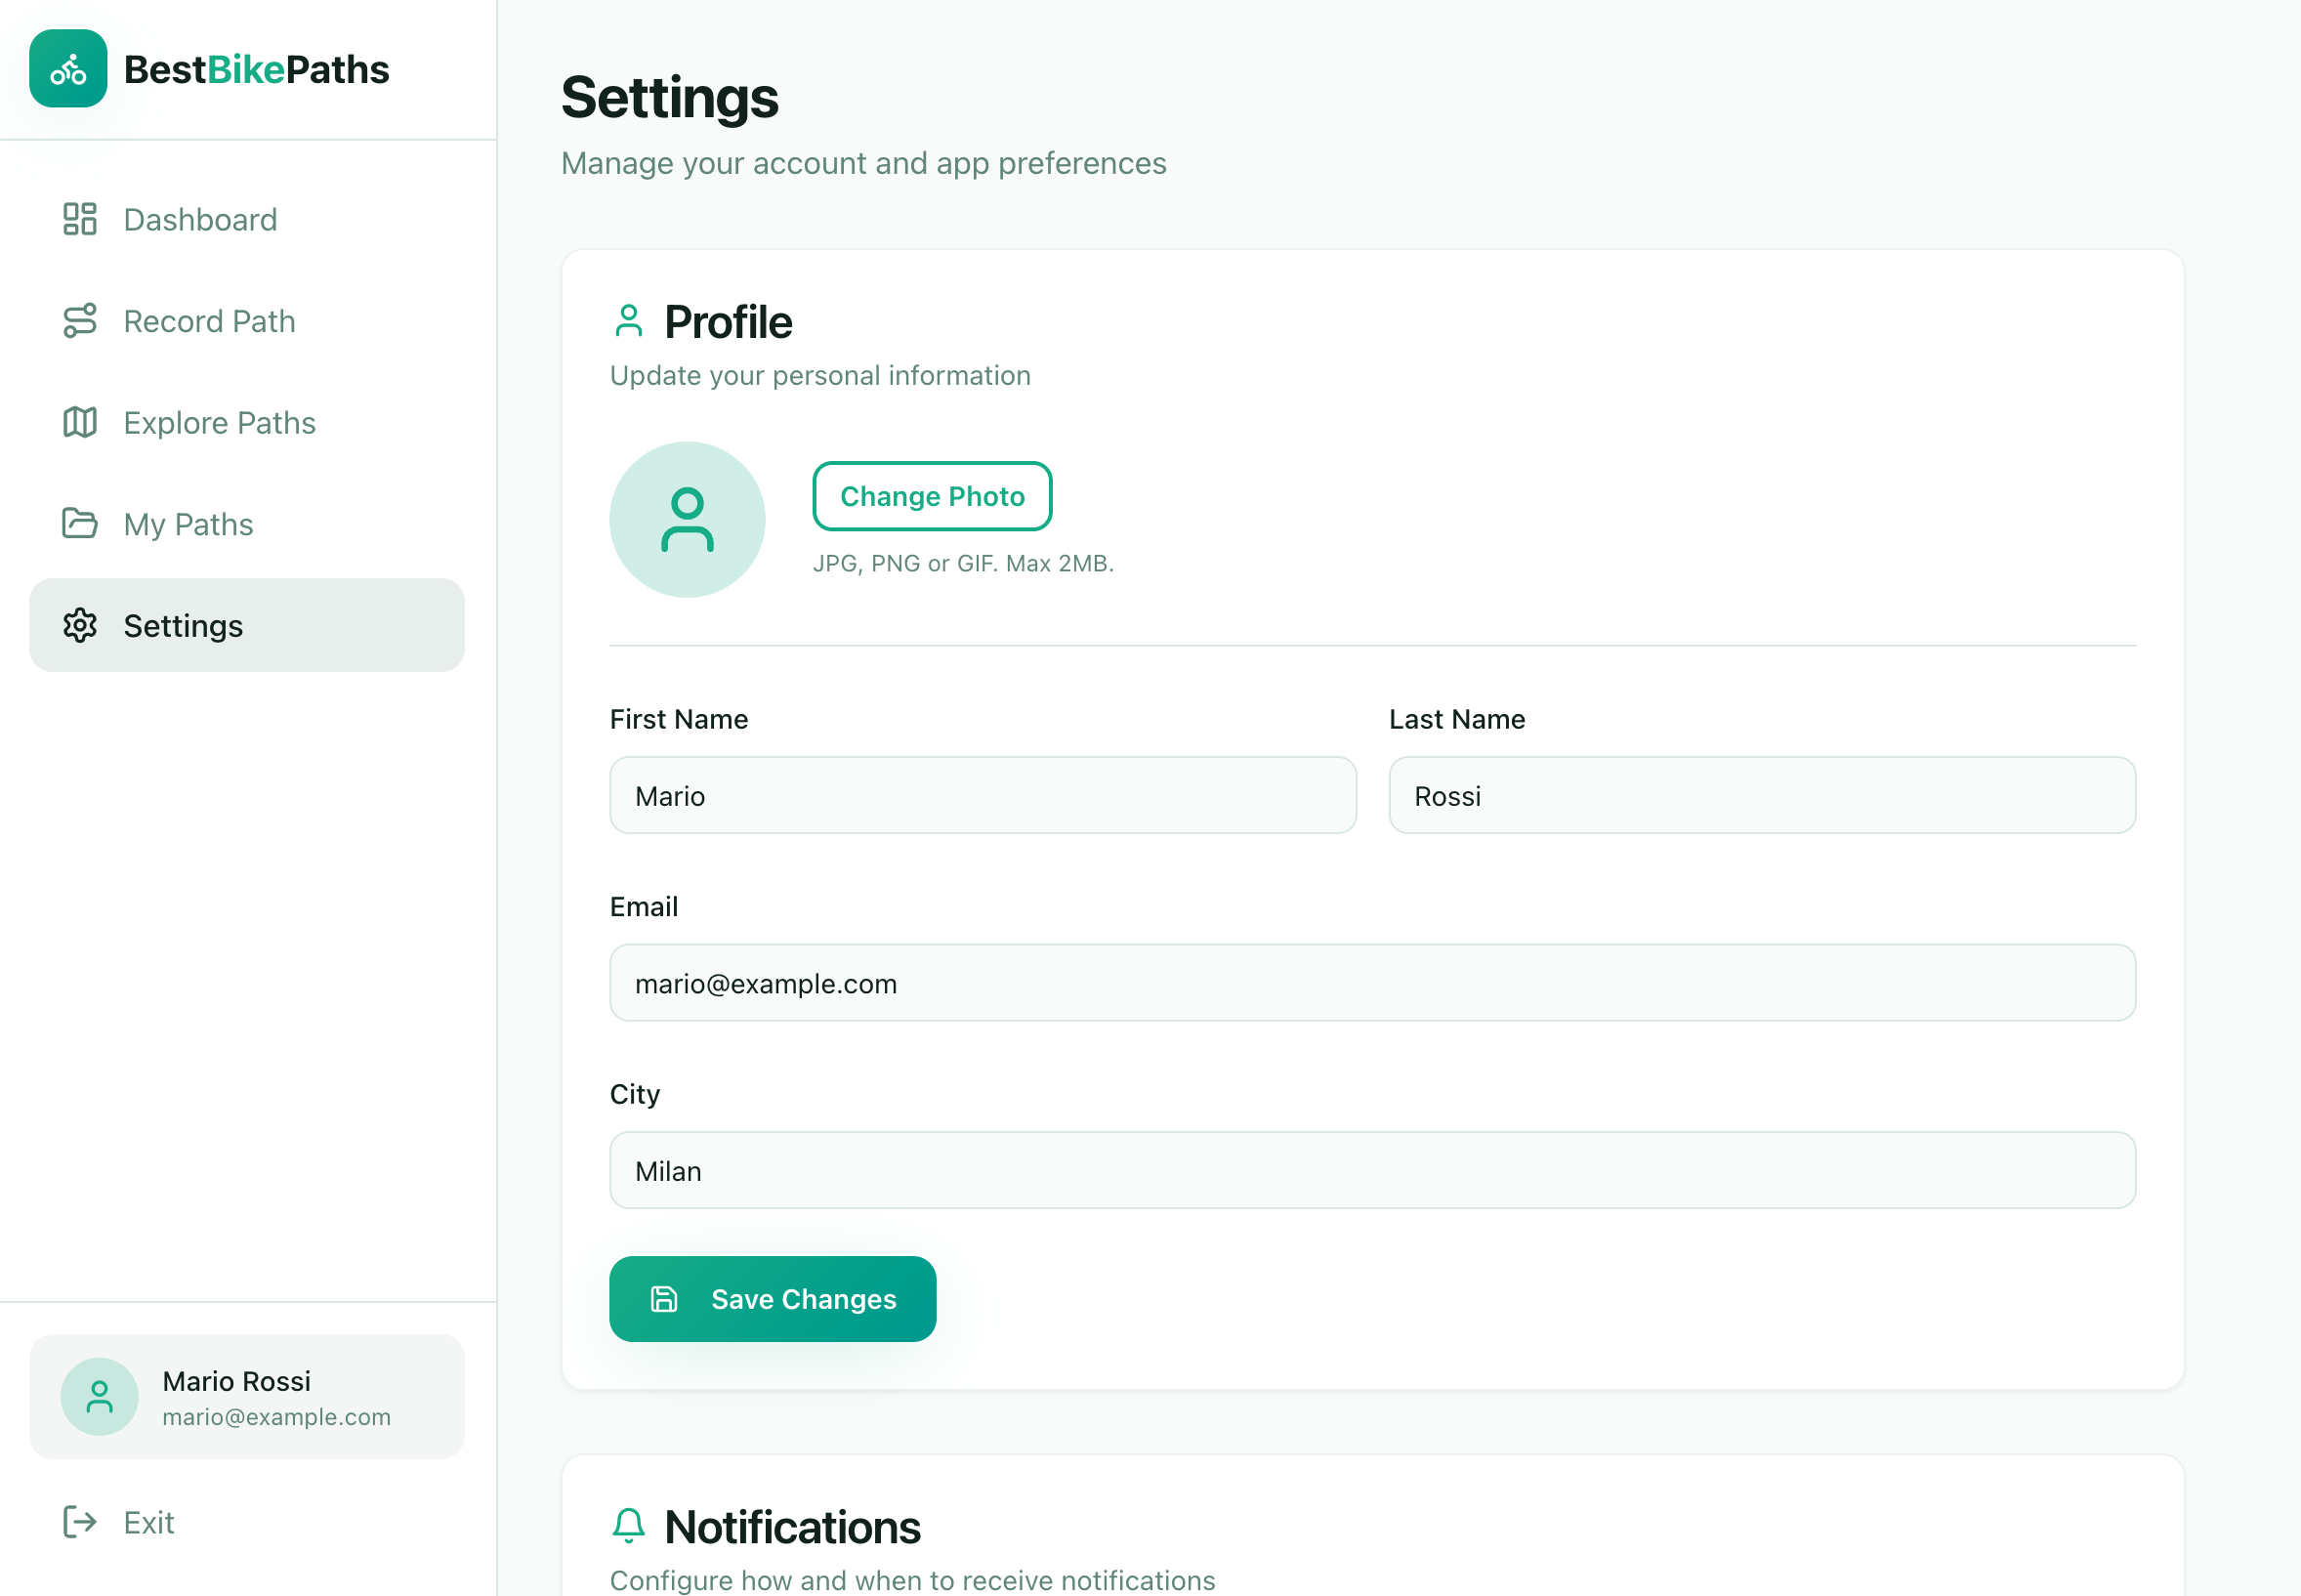
\includegraphics[width=0.25\textwidth]{Images/settings_def.png}
        \caption{Profile page}
    \label{fig:profile_page}
\end{figure}

\begin{figure}[H]
        \centering
        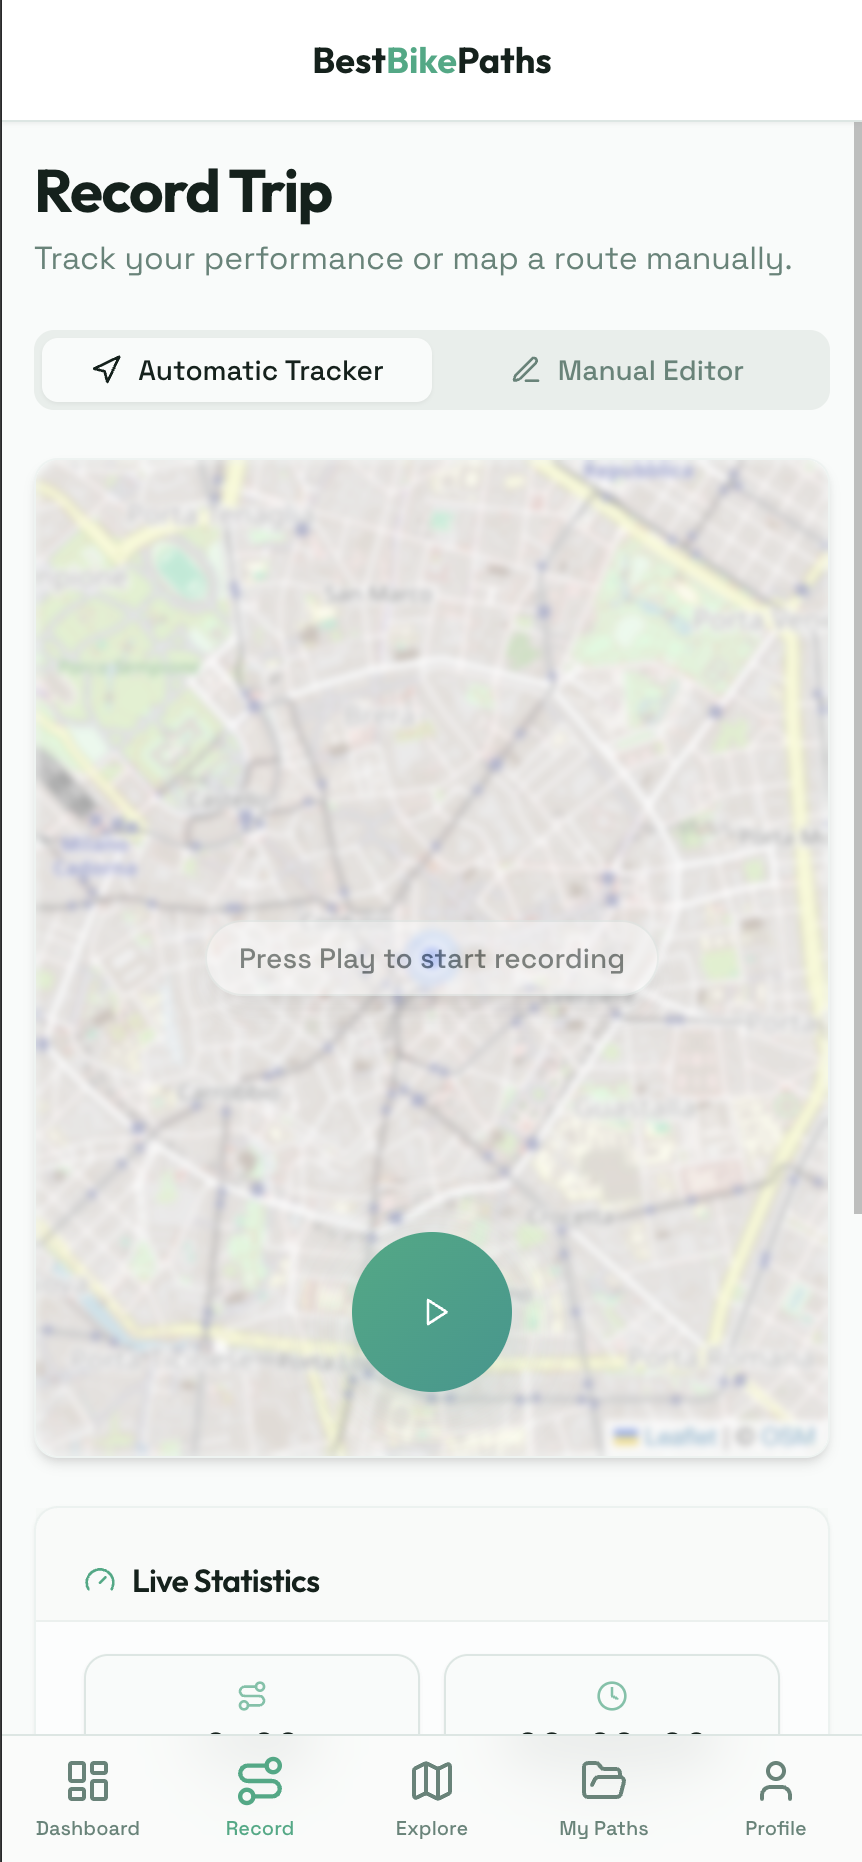
\includegraphics[width=0.25\textwidth]{Images/record_trip_def.png}
        \caption{Activity recording interface}
    \label{fig:activity_recording}
\end{figure}

\begin{figure}[H]
        \centering
        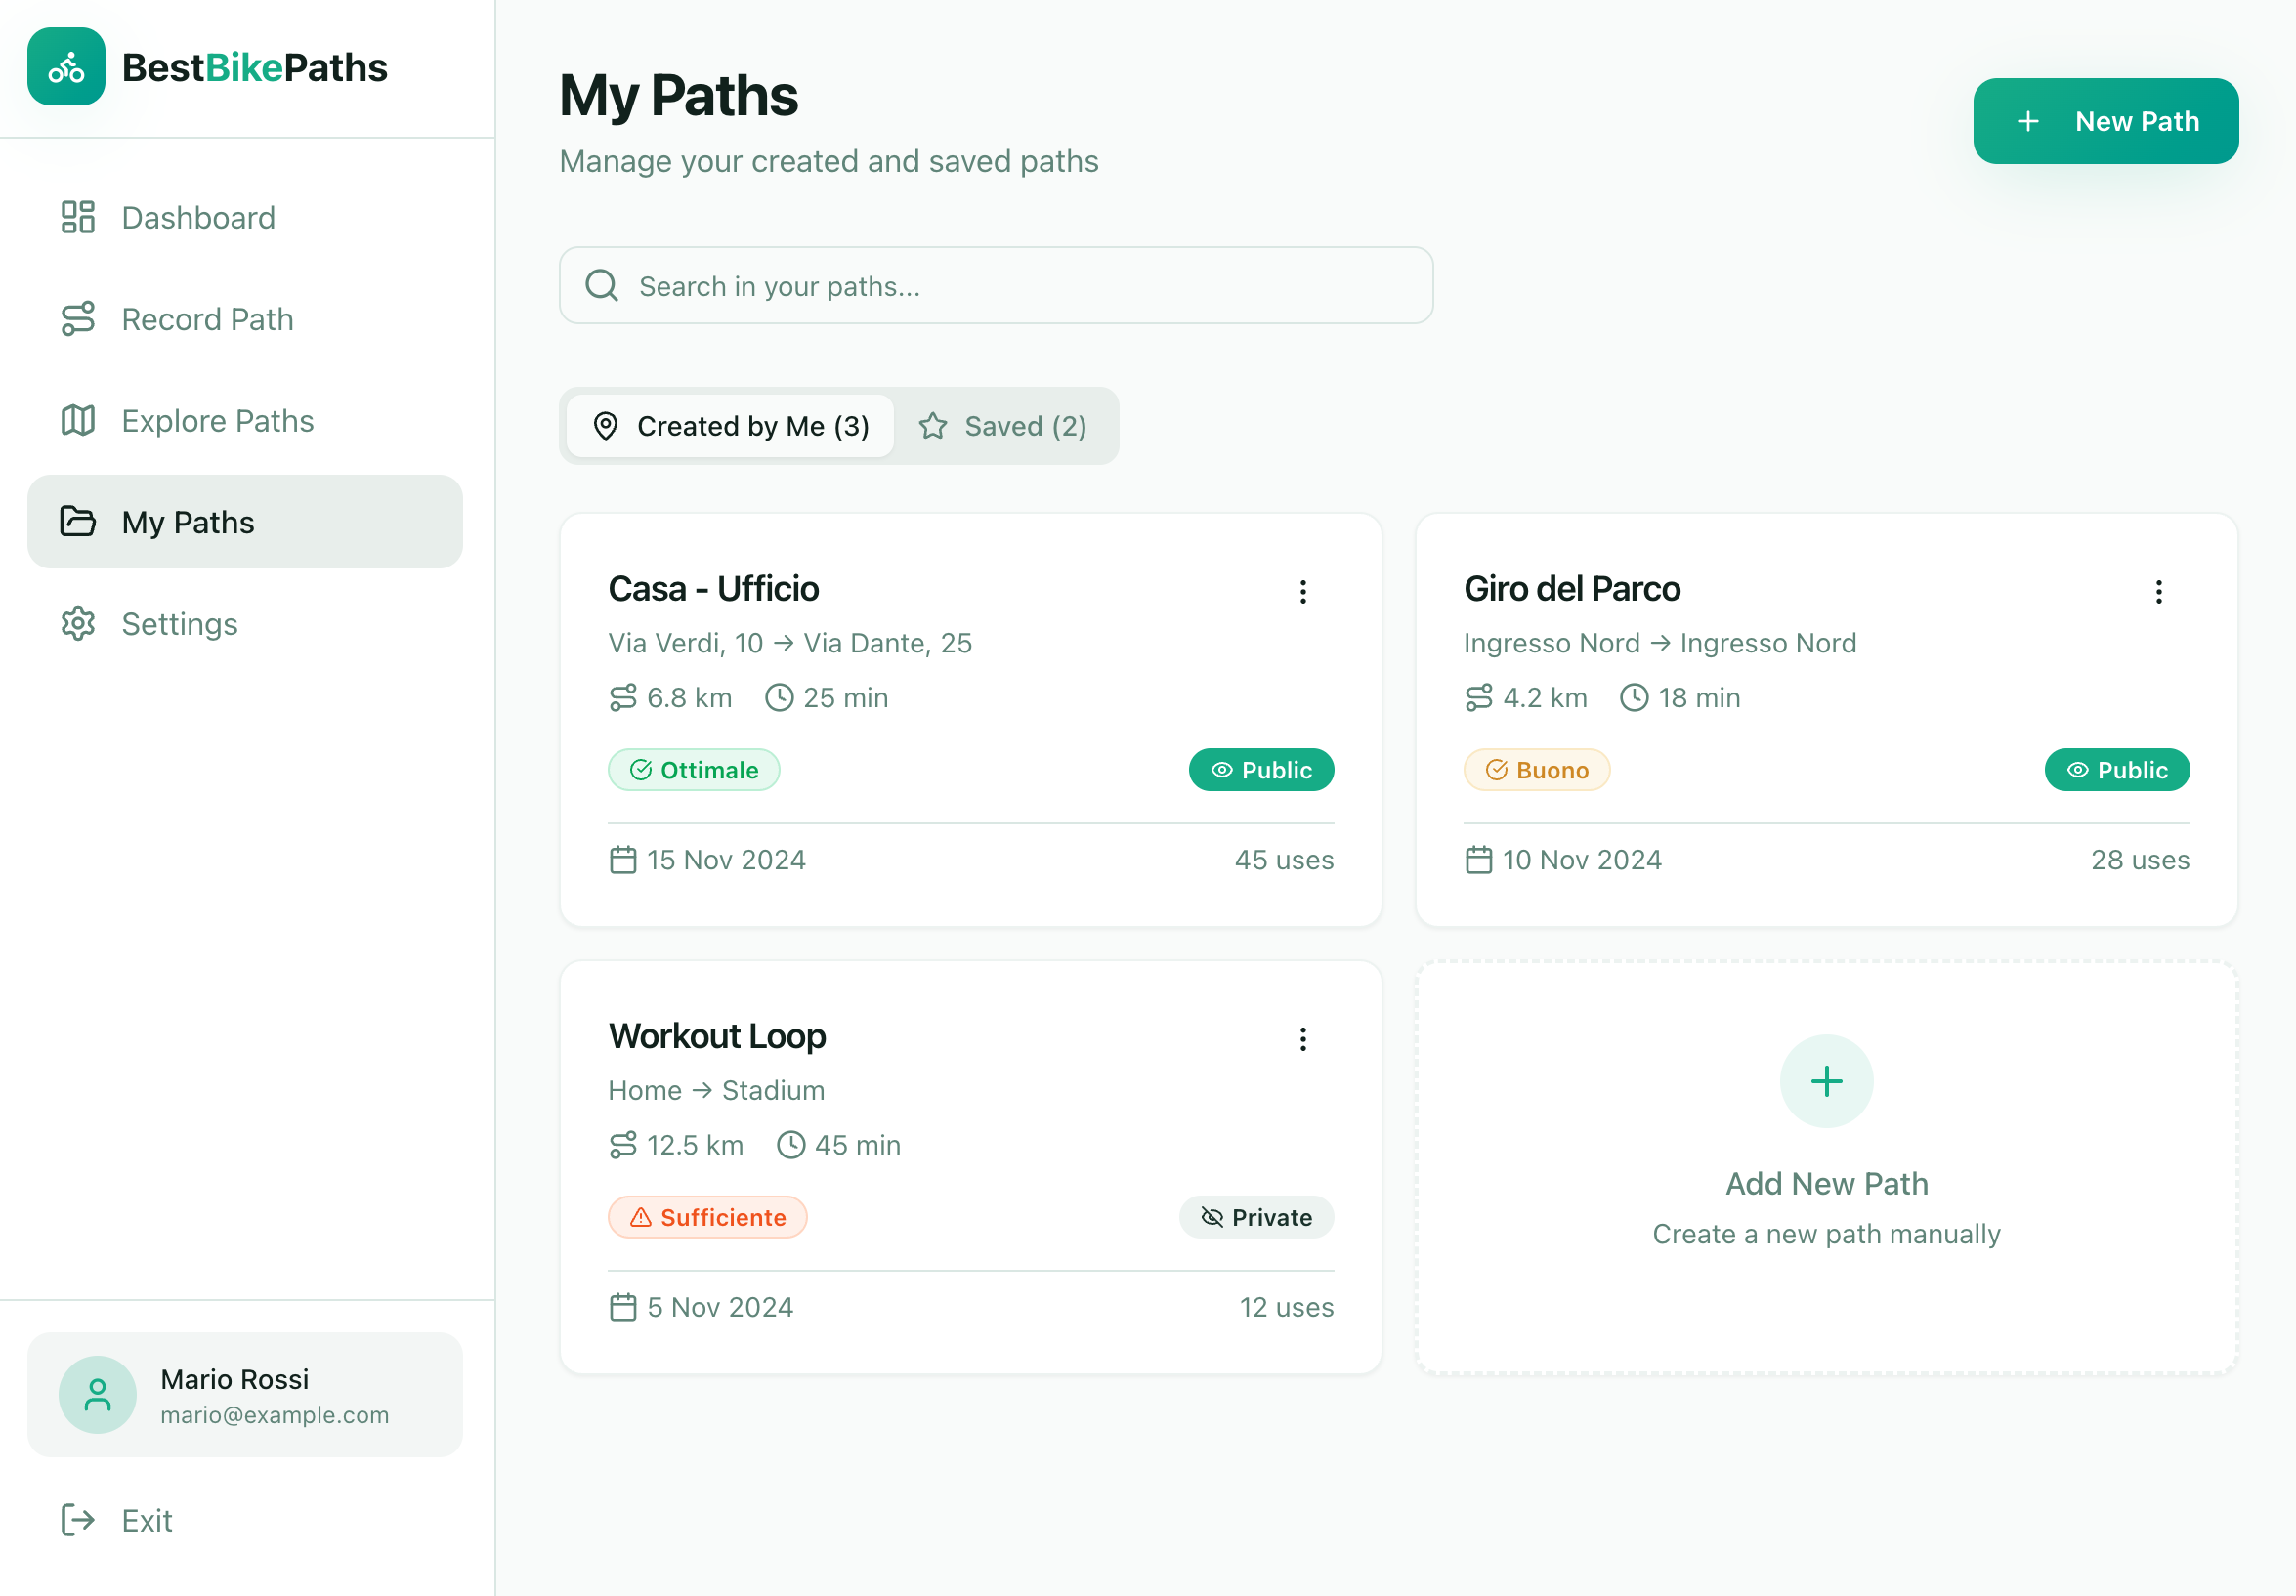
\includegraphics[width=0.25\textwidth]{Images/my_paths_def.png}
        \caption{User's personal paths}
    \label{fig:user_paths}
\end{figure}




\subsection{Hardware Interfaces}
\label{subsec:hardware_interfaces}

Since this is a web application, no additional hardware is required beyond a device capable of connecting to the internet. This applies to path browsing and manual activity creation.

However, to use the automatic recording feature, the device must include specific sensors—namely an accelerometer, GPS, and a compass.


\subsection{Software Interfaces}
\label{subsec:software_interfaces}

\begin{itemize}
    \item \textbf{Database:} To store user credentials, paths, and activities, the system must rely on a dedicated database accessible by the platform.
    
    \item \textbf{Identity provider:} The system may allow users to register with an email and password or authenticate through an external OAuth provider. This lets users access the platform without creating new credentials, using an account they already have with another service. In this case, an interface to communicate with the chosen provider is required to validate the user’s identity.
    
    \item \textbf{Meteorological data provider:} When an automatic activity is recorded, the user can enrich it with weather information retrieved from an external API. To enable this, the system must expose a secure endpoint capable of requesting and receiving accurate meteorological data.
\end{itemize}

\subsection{Communication Interfaces}
\label{subsec:communication_interfaces}

The Best Bike Paths (BBP) system is a distributed application primarily relying on a Serverless architecture (e.g., using Function as a Service, FaaS) to manage backend processing. Communication interfaces must securely handle the transmission of sensitive data (such as user location) and high volumes of telemetric data.

\begin{itemize}
    \item \textbf{User and Client-Function Communication:} All interactions between clients (web browser interfaces and mobile devices) and the backend compute layer (serverless functions) must utilize HTTPS to ensure end-to-end encryption and data security.
    
    \item \textbf{Mobile Sensor Data Transmission:} The mobile application is responsible for securely transmitting data streams from device sensors (GPS, accelerometer, and gyroscope) directly to the database. These inputs are critical for the automatic trip tracking mode and the detection of road defects (potholes). The transmission mechanism must be optimized to minimize bandwidth consumption and battery drain, utilizing efficient, asynchronous upload of collected data.
    
    \item \textbf{External Interfaces (Meteorological Service):} The BBP system interacts with an external third-party meteorological service via its public APIs (a Machine-to-Machine interface). This external interface is used by the backend functions to retrieve real-time weather data (conditions, temperature, wind speed) to enrich the saved trip data.
    
    \item \textbf{Authentication and Authorization:} User access is managed via secure mechanisms (e.g., using OAuth). These mechanisms facilitate access control to the serverless functions that manage data storage and processing, ensuring only authenticated users can access their personalized features.
\end{itemize}